% ----------------------------------------------------------
% ELEMENTOS PRÉ-TEXTUAIS
% ----------------------------------------------------------
% \pretextual

%% %%%%%%%%%%%%%%%%%%%%%%%%%%%%%%%%%%%%%%%%% %%
%% Elementos Pré Textuais
%% ----------------------
%% 
%% Devem ser os seguintes (nessa ordem):
%%  1. Capa (obrigatório)
%%  2. Folha de rosto (obrigatório)
%%  3. Errata (opcional)
%%  4. Folha de aprovação (obrigatório)
%%  5. Dedicatória (opcional)
%%  6. Agradecimentos (opcional)
%%  7. Epígrafe (opcional)
%%  8. Resumo (obrigatório)
%%  9. Abstract/Resumo em outra língua (obrigatório)
%% 10. Lista de Ilustrações (opcional)
%% 11. Lista de Tabelas (opcional)
%% 12. Lista de Abreviaturas e Siglas (opcional)
%% 13. Lista de Símbolos (opcional)
%% 14. Sumário (obrigatório)
%% %%%%%%%%%%%%%%%%%%%%%%%%%%%%%%%%%%%%%%%%% %%


% 01: Capa
\imprimircapa


% 02: Folha de rosto
% (o * indica que haverá a ficha bibliográfica)
\imprimirfolhaderosto*

%% Ficha Catalográfica
% Isto é um exemplo de Ficha Catalográfica, ou ``Dados internacionais de
% catalogação-na-publicação''. Você pode utilizar este modelo como referência. 
% Porém, provavelmente a biblioteca da sua universidade lhe fornecerá um PDF
% com a ficha catalográfica definitiva após a defesa do trabalho. Quando estiver
% com o documento, salve-o como PDF no diretório do seu projeto e substitua todo
% o conteúdo de implementação deste arquivo pelo comando abaixo:
 
    %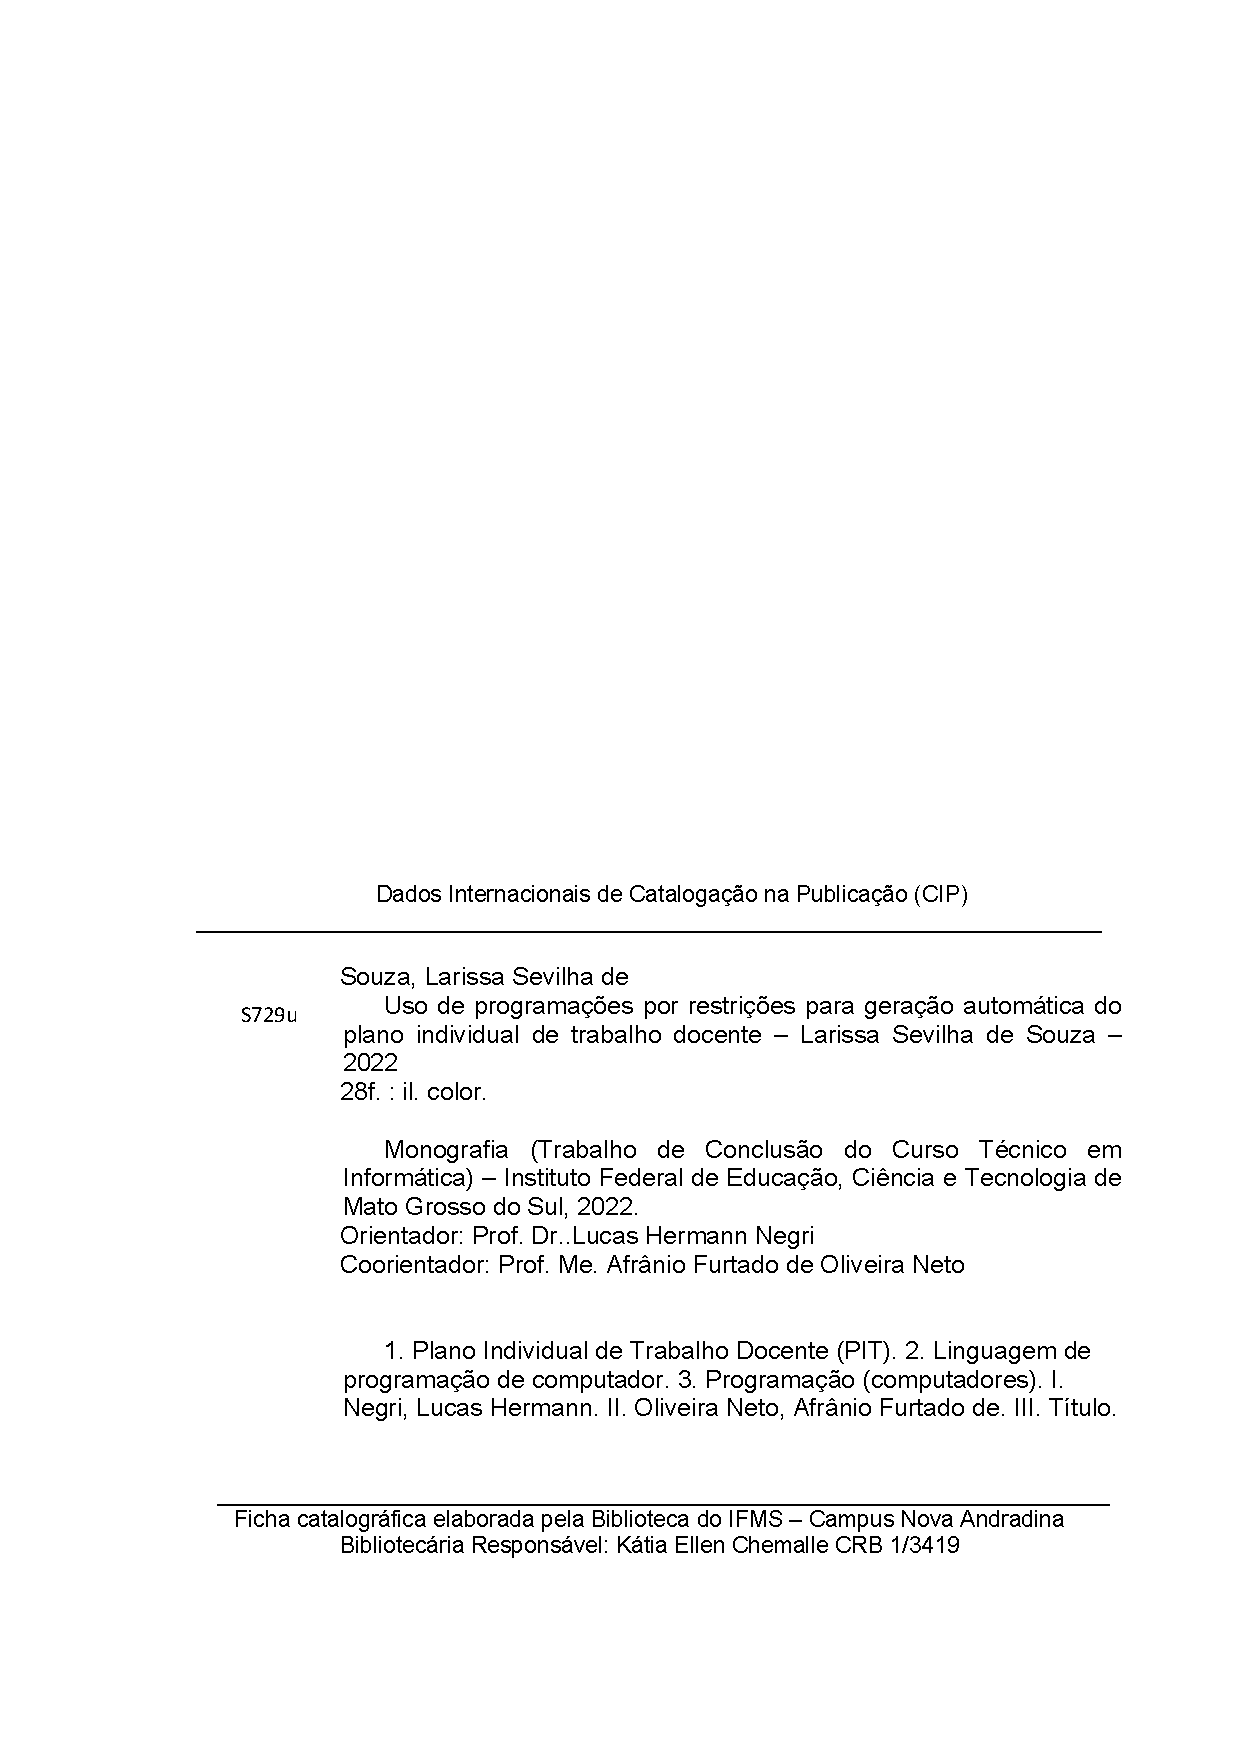
\includepdf{imagens/fichacatalografica.pdf}
 
 

% \begin{fichacatalografica}
% 	\sffamily
% 	\vspace*{\fill}					% Posição vertical
% 	\begin{center}					% Minipage Centralizado
% 		\fbox{\begin{minipage}[c][8cm]{13.5cm}		% Largura
% 				\small
% 				\imprimirautor
% 				%Sobrenome, Nome do autor
				
% 				\hspace{0.5cm} \imprimirtitulo  / \imprimirautor. --
% 				\imprimirlocal, \imprimirdata-
				
% 				\hspace{0.5cm} \pageref{LastPage} p. : il. (algumas color.) ; 30 cm.\\
				
% 				\hspace{0.5cm} \imprimirorientadorRotulo~\imprimirorientador\\
				
% 				\hspace{0.5cm}
% 				\parbox[t]{\textwidth}{\imprimirtipotrabalho~--~\imprimirinstituicao,
% 					\imprimirdata.}\\
				
% 				\hspace{0.5cm}
% 				1. Palavra-chave1.
% 				2. Palavra-chave2.
% 				2. Palavra-chave3.
% 				I. Orientador.
% 				II. Universidade xxx.
% 				III. Faculdade de xxx.
% 				IV. Título 			
% 			\end{minipage}}
% 		\end{center}
% 	\end{fichacatalografica}


% 03: Errata
% \begin{errata}
%	Elemento opcional da \citeonline[4.2.1.2]{NBR14724:2011}. Exemplo:
	
%	\vspace{\onelineskip}
	
%	FERRIGNO, C. R. A. \textbf{Tratamento de neoplasias ósseas apendiculares com
%		reimplantação de enxerto ósseo autólogo autoclavado associado ao plasma
%		rico em plaquetas}: estudo crítico na cirurgia de preservação de membro em
%	cães. 2011. 128 f. Tese (Livre-Docência) - Faculdade de Medicina Veterinária e
%	Zootecnia, Universidade de São Paulo, São Paulo, 2011.
	
%	\begin{table}[htb]
%		\center
%		\footnotesize
%		\begin{tabular}{|p{1.4cm}|p{1cm}|p{3cm}|p{3cm}|}
%			\hline
%%			\textbf{Folha} & \textbf{Linha}  & \textbf{Onde se lê}  & \textbf{Leia-se}  \\
%			\hline
%			1 & 10 & auto-conclavo & autoconclavo\\
%			\hline
%		\end{tabular}
%	\end{table}
	
\end{errata}


% 04: Folha de Aprovação
% Isto é um exemplo de Folha de aprovação, elemento obrigatório da NBR
% 14724/2011 (seção 4.2.1.3). Você pode utilizar este modelo até a aprovação
% do trabalho. Após isso, substitua todo o conteúdo deste arquivo por uma
% imagem da página assinada pela banca com o comando abaixo:
%

%Colocar ata da defesa

%

%\imprimirfolhadeaprovacao

%% Use esta se forem 4 membros na banca:
%\imprimirfolhadeaprovacaoduascolunas

% \includepdf{folhadeaprovacao_final.pdf}



%% 05: Dedicatória
\begin{dedicatoria}
   \vspace*{\fill}
   \centering
   \noindent
 %  \textit{ Este trabalho é dedicado às crianças adultas que,\\
  % quando pequenas, sonharam em se tornar cientistas.} \vspace*{\fill}
\end{dedicatoria}


%% 06: Agradecimentos
%\begin{agradecimentos}

%\end{agradecimentos}


%% 07: Epígrafe
% \begin{epigrafe}
	\vspace*{\fill}
	\begin{flushright}
	%	\textit{``Não vos amoldeis às estruturas deste mundo, \\
	%		mas transformai-vos pela renovação da mente, \\
	%		a fim de distinguir qual é a vontade de Deus: \\
	%		o que é bom, o que Lhe é agradável, o que é perfeito.\\
	%		(Bíblia Sagrada, Romanos 12, 2)}
	\end{flushright}
\end{epigrafe}


%% 08: Resumo
\setlength{\absparsep}{18pt} % ajusta o espaçamento dos parágrafos do resumo
\begin{resumo}
    A crescente aplicação de tecnologias de automação em ambientes residenciais tem impulsionado o desenvolvimento de sistemas voltados à otimização de tarefas cotidianas. Neste contexto, o presente trabalho propõe o desenvolvimento de um sistema automatizado para limpeza e manutenção de piscinas residenciais, fundamentado em princípios de automação residencial e na Internet das Coisas (IoT).

    sistema integra sensores, atuadores e controladores microprocessados com o objetivo de realizar o monitoramento e o tratamento automatizado da água, reduzindo a necessidade de intervenção manual.
    
    A proposta busca oferecer maior eficiência no uso de recursos, segurança na manipulação de produtos químicos e sustentabilidade no consumo de água e energia. A pesquisa abrangeu a revisão de normas técnicas, o estudo dos componentes mecânicos e eletrônicos empregados, bem como o desenvolvimento de um protótipo funcional.
    
    Os resultados obtidos demonstram que a automação do processo de limpeza e tratamento de piscinas é viável e pode minimizar falhas humanas, otimizar o tempo de manutenção e garantir padrões adequados de qualidade da água. O sistema desenvolvido apresenta-se, portanto, como uma solução prática e acessível, alinhada às tendências tecnológicas de domótica e automação inteligente.

	\textbf{Palavras-chave}:  Automação residencial. IoT. Piscinas residenciais. Manutenção automatizada.
\end{resumo}


%% 09: Abstract/Resumo em língua estrangeira
% resumo em inglês
\begin{resumo}[Abstract]

\begin{otherlanguage*}{english}

Considering the repetitive work involved in the development of the Teacher Work Plan (TWP) in the Federal Institute of Mato Grosso do Sul (IFMS), an automated method is proposed for building an optimized TWP by using constraint programming.

The method is implemented with the Google OR-Tools library and is modeled after on built in mandatory constraints and teacher preferences that are described as the program input.

A graphical interface was developed using JavaScript, JQuery, HTML and CSS to make the system more user-friendly.

The method was evaluated using a real teacher situations, where an idea of the efficiency and performance of the method could be evaluated. Results showed that the method was able to build the timetable according to the rules and preferences of the teacher, minimizing the exchange of activities and free time between them.

		\vspace{\onelineskip}
		
		\noindent 
		\textbf{Keywords}: constraint programming, scheduling, optimization.
	\end{otherlanguage*}
\end{resumo}


%% 10: Lista de Ilustrações
%\pdfbookmark[0]{\listfigurename}{lof}
%\listoffigures*
%\cleardoublepage


%% 11: Lista de Tabelas
%\pdfbookmark[0]{\listtablename}{lot}
%\listoftables*
%\cleardoublepage


%% 12: Lista de Abreviaturas e Siglas
%\chapter{}


%% 13: Lista de Símbolos
% %\chaopter{}


%% 14: Sumário (o asterisco retira o próprio sumário do sumário)
\pdfbookmark[0]{\contentsname}{toc}
\tableofcontents*
\cleardoublepage
